
\chapter{Thirukkural and its affiliation to Sanātana Dharma}\label{chap04}

\Authorline{A.V. Gopala Krishnan (Devapriyaji)}


\section*{Abstract}

Tamil\index{Tamil} with an unbroken literary history of over two millennia, has produced many a literary gem and the foremost among them is Thirukkuŗal\index{Thirukkural@Thirukkuŗal} (Sacred Couplets), attributed to Thiruvalluvar\index{Thiruvalluvar}.

Valluvar was considered a Brahmin when the picture was requested for Stamp release by Central Govt in 1963.

Christian Church made generous funding to claim Thirukkural as a Christian work – this was later examined and more reputed Christian Scholars have rejected the 100\% Church funded Doctorates.

Speculation that Thirukural was a Jain\index{Jain} work mainly started in the 19th century, but is still repeated by many scholars mostly aligned with Communist or Dravidian ideologies. This is repeated in several literary meets and Universities.

This paper analyses Thirukkural completely and finds that there is not one verse in support of these claims. It finds Kural teachings concerning ascetics are totally against Jain \textit{Yati Dharma} for monks.

Valluvar mostly uses only titles of attributes to God and not names in First Chapter; references in Tamil Thesaurus (\textit{Nigandu-}s\index{Nigandu@\textit{Nigandu}}) most of them belonging to end 10th century or later, to Jain Tirthankara-s, have been extensively relied upon to make the above claim. However a few of these titles for Vedic Gods have been used much earlier in Sangam literature and also by 7th century CE Śaiva poet Gnanasambanthar, for Lord Shiva.\index{Sambandhar}

We also analyze Valluvar’s teaching for a just reign and unjust reign by the king for the glory of Vedas.

While Kuŗal is life-affirming, Jainism is life-denying. Valluvar talks of God Almighty the creator God, not Gurus or Tirthankara-s of Jainism, who do not accept Creator God. Valluvar used names of twenty-five Hindu Gods in various Kurals.

Thiruvalluvar’s work is not a religious treatise, but a book to teach virtues and from analyzing various verses throughout 1330 verses, any honest person would accept that Kural is very close to \textit{Sanātana Dharma}\index{Sanatana Dharma@\textit{Sanātana Dharma}} and \textit{Dharma Śāstra-s.}\index{Dharma Sastra@\textit{Dharma Śāstra}}


\section*{1 Tirukkural - an Introduction:}

Tamil with an unbroken literary history of over two millennia, has produced many a literary gem and the foremost among them is Thirukkuŗal (Sacred Couplets), attributed to Thiruvalluvar.

Thirukkural, on its poetical merit, ethical values and overwhelming popularity, continues to attract the attention of scholars to write commentaries and produce new translations in different languages. The holistic nature of the work meant that it has attracted the attention of all scholars irrespective of their religious affiliations. A concerted attempt to call it a Jaina work is analyzed here.

Thirukkural was originally called Muppāl\index{Muppal@Muppāl} (3 Sections) with 133 Chapters having 10 verses in each, totalling 1330 verses. The three sections are as given below.

\begin{enumerate}[{\rm 1)}]
\itemsep=0pt
\item Dharma (Aram) - 38 Chapters

 \item Artha (Porutpal) - 70 Chapters

 \item Kāma - 25 Chapters

\end{enumerate}

\newpage

The overall organization of the Kural text is based on seven ideals prescribed for a commoner, besides observations on love. The division of topics may be understood as follows.

\begin{itemize}
\item 40 couplets on God, rain, ascetics, and virtue

 \item 200 couplets on domestic virtue

 \item 140 couplets on higher yet most fundamental virtue based on grace, benevolence and compassion

 \item 250 couplets on royalty

 \item 100 couplets on ministers of state

 \item 220 couplets on essential requirements of administration

 \item 130 couplets on morality, both positive and negative

 \item 250 couplets on human love and passion

\end{itemize}

\textbf{Thirukkural follows the pattern of Dharma- Artha- Kāma of Vedic tradition, leaving Mokṣa which is the goal of every chapter- he says in his first Chapter (last Kural 10) - “where none can swim the great sea of birth but those who are united with the feet of God".}

Thirukkural is dated around the latter part of 3rd or early 4th century CE by scholars based on use of words which belong to later than Sangam\index{Sangam} literature and also on other references. The Tamil epic \textit{Silapathikāram} and the Grammar treatise Tholkāppiyam\index{Tholkappiyam@Tholkāppiyam} are later than this. Thirukkural, in the history of Tamil Literature, has been regarded as teaching the righteousness, \textit{dharma}, dealing with the everyday virtues of an individual as explained in Veda-s and Smŗti-s.


\section*{2 Thiruvalluvar - Author of Thirukkural}

Thirukkural does not have its author’s name, and its dating is based on later works only. \textbf{Thiruvalluva Malai}\endnote{Book analyses various stories about Valluvar: - Sundaram, Dr.Shanmuga (1985) \textit{ValluvarkaL. }Bengaluru: Kaavya Publishers} is a collection of songs praising and giving details of Thirukkural. Written by 55 poets, most of the authors named are similar to those of Sangam Literature, but research indicates that some songs belong to late First Millienium and some to the 16/17th century CE.

Many stories and details about Valluvar’s life have been created much later and no reliable information is available. Christian missionaries\endnote{Blackburn, Stuart (2000) “Corruption and Redemption: The Legend of Valluvar and Tamil Literary History”. \textit{Modern Asian} \textit{Studies}. 34(02).April 2000. Pp. 449-482.} have contributed many tales which have no historical value, to confuse the public.

A collection of a few later songs say that Valluvar\index{Valluvar} was born in a lower caste of the fourth varņa - but clearly the use of language and style proves Christian\endnote{As above} hand in it.

\subsection*{Tirukkural and Valluvar in Tamil Society}

Thirukkural has been called in various names as follows.

\tamil{முப்பால்} (\textit{Muppāl}\index{Muppal@\textit{Muppāl}}) – “The three-sectioned" or “The three-fold path" (Original name given by Valluvar)

\tamil{பொய்யாமொழி} (Poyyāmoḻi) – “Statements devoid of untruth"

\tamil{உத்தரவேதம்} (Uttaravedam) – “Highest Veda"[14]

\tamil{வாயுறை வாழ்த்து} (Vāyurai Vāḻttu) – “Truthful utterances"

\tamil{தெய்வநூல்} (Teyvanūl) – “The holy book"

\tamil{பொதுமறை} (Potumaṟai) – “The universal Veda" or “Book for all"

\tamil{தமிழ்மறை} (Tamiḻ Maṟai) – “The Tamil Veda"

\tamil{முப்பானூல்} (Muppāṉūl) – “The three-sectioned book"

\tamil{ஈரடி நூல்} (Iradi ṉūl) – “The two-lined book"

\tamil{வள்ளுவம்} (Valluvam) – “Valluvarism" or “The work of Valluvar" and held high in Tamilnadu.

Earliest missionaries who came to Tamilnadu were advised to read Kural, along with other books such as Ramāyaņa\index{Ramayana@Ramāyaņa} etc., which shows that Tamil society held Kural as an important work that teaches Vedic principles.

Earliest references to Kural all speak of it as the Tamil manifestation of Vedas. Both Silappathikāram\index{Silappathikaram@Silappathikāram} and Maņimekalai\index{Manimekalai@Maņimekalai} use the reference, but do not say that it follows Jainism or Buddhism. Śaiva Siddhānta\index{Saiva Siddhanta@Śaiva Siddhānta} has been claiming Kural\index{Kural} as their book for more than 700 years and a Śaiva temple for Valluvar exists in Mylapur\endnote{\url{ https://en.wikipedia.org/wiki/Thiruvalluvar_Temple} as viewed on\break 09.01.2017} dating from the 14th century CE.

There are a few more works in the name of Poet Valluvar, but literary research based on the words used indicates that they are from different authors\endnote{\url{ https://en.wikipedia.org/wiki/Thiruvalluvar} as viewed on 09.01.2017} and belong to 16the Century or later.


\subsection*{Tiruvalluvar Coin \& Stamp}

The Government of India released a stamp and Coin to commemorate Tiruvalluvar in 1963.\endnote{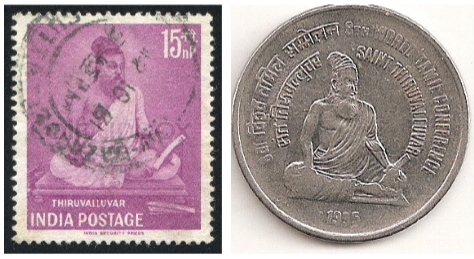
\includegraphics[scale=0.4]{images/art04-fn-6.jpg}}


\subsection*{Tirukkural – General Opinion}

Written for the purpose of teaching ethics, Tirukkural expounds a universal moral and practical attitude towards life. Tirukkural refrains from talking of hopes and promises of the other-worldly life. Rather it speaks of the ways of cultivating one's mind to achieve the other-worldly bliss in the present life itself. By occasionally referring to bliss beyond the worldly life, Valluvar equates what can be achieved in human life with what may be attained thereafter.

As Valluvar did not use any direct names for God in the first chapter “In Praise of God” it is more easily accepted by believers of all faiths and many Tamil organisations want Thirukkural be declared as “Universal Scripture” (Ulagap pothumarai).


\section*{3 Tirukkural as a Christian Work - forgery that went to Court}

G.U. Pope in his Translation of Kural to English, says in his Introduction that Kural would not have been written without the knowledge of Christian Bible, and that Valluvar lived in Mylapur on the coast, would have had connection with Christian travellers by sea. He also speaks of another possibility of St. Thomas\index{St. Thomas}, disciple of Jesus preaching in Chennai, meeting Valluvar. Earliest to record all this is Ishwar Charan\endnote{\url{ https://ishwarsharan.wordpress.com/}} “The Myth of Saint Thomas and the Mylapore Shiva Temple” 1991 and revised edition in 2010 and also Vedaprakash in Tamil \tamil{“இந்தியாவில் செயின்ட் தாமஸ் கட்டுக் கதை”}

This concept was developed by a tie-up of Roman Catholic San Thome Church\index{San Thome Church} with Protestant Madras Christian College\endnote{\url{ https://ta.wikisource.org/s/42n1 }}, a First Book published in 1969- “\textit{Thiruvalluvar Christhuvaraa}” with a foreword from then Chief Minister \textit{M. Karunanithi}\index{Karunanithi, M.@\textit{Karunanithi, M.}}\endnote{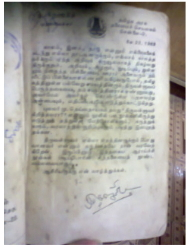
\includegraphics[scale=0.4]{images/art04-fn-9.jpg}}. The book made extremely new claims as explained below.

Page 31\endnote{\tamil{“வள்ளுவர் காப்பியடித்தார் எனக் கூற எந்தத் தமிழனும் முன் வர மாட்டான். ஆனால் விறுப்பு, வெறுப்பின்றி ஆய்பவர்கள் தங்கள் ஆய்வின் முடிவில் வரும் கருத்துக்களை வெளியிடப் பின் வாங்கினால் அவர்கள் உண்மை ஆய்வாளார் அல்லர்.} –Page31 \tamil{“திருவள்ளுவர் கிறித்தவரா?”}} -- “No Tamil would like to say that Valluvar copied his work from other sources, but if a researcher at the end of his true research without favour or pre-opinion should reveal the truth.” (translated from Tamil) 

Page 73\endnote{\tamil{“கிறித்தவமாகிய மலையிலிருந்து எடுக்கப்பட்ட அறமாகிய கருங்கல், தமிழாகிய கங்கையில் நீராட்டப்பட்டு திருக்குறளாம் பேசும் சிற்பம் தோன்றியது. தோமையரின் மூலம் பெற்ற நற்செய்தியாம் அறத்தை தன் அரசியல் பணியிலிருந்து பெற்ற அரசியலறிவாம் பொருளுடன், தன் இல்வாழ்வின் அடித்தளத்தில் விளங்கிய இன்பத்தோடு சேர்த்துத் தமிழ்ச் சூழலில் முப்பாலாக மொழிந்துள்ளார்.} Page- 73 - \tamil{“திருவள்ளுவர் கிறித்தவரா? “}} -- “From the Mountain called Christianity\index{Christianity} – the stone of Dharma was taken and after dipping it in Ganges of Tamil came Thirukkural the Speaking Sculpture. From the Gospel of Dharma from St.Thomas – Valluvar who was a minister in Politics with his political knowledge and his rich family life brought “The three-sectioned".” (translated from Tamil)

It faced little resistance. Then later several small books on various virtues which were advocated by Valluvar, but not in agreement with Bible, appeared, misinterpreting the verses using 20th century Commentaries of various followers of Dravidian ideology.

\textbf{Church became so confident that Thiruvalluvar} could be called Christian and Kural as Christian book that it arranged a Forger to make “Fake Ancient Manuscripts for Kural with Christian meanings” and One Acharya Paul Ganesh Iyer\endnote{ Archbishop Arulappa Sends His Document Forger To Jail – Ganesh Iyer \&amp; K.P. Sunil \url{https://ishwarsharan.wordpress.com/parts-2-to-9/archbishop-arulappa-sends-his-document-forger-to-jail-ganesh-iyer-k-p-sunil/ }} was given money in several Lakh Rupees and taken on an international trip including a 20-minutes session with Pope. The Church realized being caught filed a case and after conviction\endnote{ Archbishop Arulappa’s History Project Goes Terribly Wrong – K.P. Sunil \url{https://ishwarsharan.wordpress.com/parts-2-to-9/archbishop-arulappas-history-project-goes-terribly-wrong-k-p-sunil/}} – made an out of court compromise allowing the person to retain his immovable properties.

Church still proceeded in academic activities – \textbf{created 100\% funded “Tamil Christian Department”} in Madras University\endnote{\url{ http://www.unom.ac.in/uploads/miscelloneous/schools/religious/christian_studies.pdf }} which is still working and \textbf{several Doctorates\supskpt{\endnote{\tamil{பி.எச்டி. வாங்கலியோ பி.எச்டி.! சாந்தோம் சர்ச்} \url{ https://saintthomasfables.wordpress.com/2010/05/24/santhome-p-hd/ }}} have been awarded for development of Thoma vazhi Christianity} which meant “Hinduism is an offshoot of Thomas Christianity”.

The main work “Viviliyam – Thirukkural – Śaiva Siththantham- a comparison”\endnote{\tamil{விவிலியம் திருக்குறள் சைவசித்தாந்தம் ஓர் ஒப்பாய்வு}} in the name of Dr. M. Deivanayagam, says very clearly “in all my works I am indebted to Santhome Church Archbishop Dr. Arulappa for Monetary and Literary assistance.”

\subsection*{Impartial Christian Scholars Deny Thirukkural Being a Christian Book}

Valluvar describes Human Life as Sea of births and the purpose of education as

356 \tamil{கற்றீண்டு மெய்ப்பொருள் கண்டார் தலைப்படுவர் மற்றீண்டு வாரா நெறி} “Who learn, and here the knowledge of the true obtain, Shall find the path that \textbf{hither cometh not again.}” Christianity does not believe in repeated births and Valluvar says it is like sleeping and waking up we are born again and again. (Kural 339)

Scholars sponsored by the Church changed the meaning of Kural and misused verses of the Bible.

Madurai Kamarajar University’s Kural Peedam established by\break Mu.Varadarajanar selected \textbf{Lecturer Selvi. Kamatchi Sinivasan}, who was born in a Saivite family in Srilanka, came to India and had served in various colleges before joining the Kural Peedam. She had \textbf{converted to Christianity} also. She was of highest repute for integrity and Peedam asked her to bring out a number of books; two had titles \textbf{“Thirukural and Bible”} and \textbf{“Religion of Thirukural”}. Her books were published posthumously by the Peedam, her views represented by a team of experts who prepared the final edition.

The Author was selected for her strict integrity, being a Christian Convert. Finally looking at the methods adopted by M. Deivanayagam,\index{Deivanayagam, M.} the learned author says\endnote{\tamil{“மு.தெய்வநாயகத்தின் நூல்களைப் படிக்கும்போது அவர் திருக்குறளைச் சரியாக புரிந்து கொண்டாரா என்பதனுடன் கிறிஸ்தவ சமய வரலாற்றையும் எவ்வளவு கற்றறிந்தார் என்ற ஐயமே ஏற்படுகிறது. – குறள் கூறும் சமயம்// குறள் கூறும் சமயம்} Page -216} – \textbf{“from the works of Deivanayagam, it is doubtful whether he understood Thirukkural or for that matter Deivanayagam’s credentials in understanding the history of Christianity is doubtful.”}

Rev. \textbf{S.J. Rajamanikam\index{Rajamanikam, S.J.} was the Head of Tamil Dept., Loyala College}\endnote{\tamil{திருக்குறளில் கிறித்தவம்-மெய்த்திரு (டாக்டர்) எஸ். இராச மாணிக்கம்,} S.J. \tamil{கத்தோலிக்க லயோலா கல்லூரித் தமிழ்த்துறை தலைவர் “ நிற்க. தற்போது ‘தெய்வநாயகம்’ என்ற புலவர் ‘திருவள்ளுவர் கிறித்தவர்’ என்று கூறி, கிறித்தவத்துக்கு முரணாகத் தென்படும் பல குறளுக்குப் புதிய விளக்கம் கூறி வருகிறார். மேலும்,} 1. \tamil{‘திருவள்ளுவர் கிறித்தவரா?} 2. \tamil{ஐந்தவித்தான் யார்?} 3. \tamil{வான்} 4. \tamil{நீத்தார் யார்?} 5. \tamil{சான்றோர் யார்?} 6. \tamil{எழு பிறப்பு} 7. \tamil{மூவர் யார்?} 8. \tamil{அருட்செல்வம் யாது? என்ற பல நூல்களை வெளியிட்டிருக்கிறார். அவற்றுள் சிலவற்றை ஊன்றிப் படித்தும், அவர் வலியுறுத்தும் கருத்தை நம்மால் ஒப்புக் கொள்ள முடியவில்லை. ‘திருவள்ளுவர் மறுபிறப்பை ஏற்கவில்லை’ என்றும், ‘ஐந்தவித்தான் என்பான் கிறித்து’ என்றும், ‘வான் என்பது பரிசுத்த ஆவி’ என்றும், நித்தார் என்பவர் கிறித்து பெடுமானார்’ என்றும், ‘சான்றோர் என்பது கிறித்தவர்களைச் சுட்டுகின்றது’ என்றும் பல சான்றுகளால் அவர் எடுத்துரைக்கின்றார்.}

\tamil{இக்கருத்துக்களோ, அவற்றை மெய்ப்பிக்க அவர் கையாளும் பலச் சான்றுகளோ, நமக்கு மனநிறைவு அளிக்கவில்லை. கிறித்துவ மதத்துக்குரிய தனிச்சிறப்பான கொள்கை ஒன்றும் திருக்குறளில் காணப்படவில்லை.} pages92-93- from \tamil{திருக்குறள் கருத்தரங்கு மலர்}-1974,(Thirukural Karuththarangu Malar-1974) Edited by Dr.N.Subbu Reddiyar}, and he was asked to present a Paper on – Presence of Christianity in ThiruKural in 1974, at Venkateshwara University – Tirupathi in Tamil\index{Tamil}; here Learned Scholar explains the ideals of Valluvar and how it varies with the important ideals of Christianity- stated in a paper that the methods used in Deivanayagam’s method are dubious and not convincing and he does not find Christian ethics in Kural. He also referred to the fact that Tiruvalluvar used names of Hindu Gods in more than twenty occasions in various Kurals but not a single Christian one.

Trichy \textbf{Bishop Heeber College Head of Department of Tamil -\break Dr.P.S. JESUDASAN} wrote a book titled \textbf{“Thirukuralum Thiruvi\-viliyamum”}\endnote{\tamil{ப.ச.ஏசுதாசன், முன்னாள் திருச்சி பிஷப். ஹீபர் கல்லூரி துணை முதல்வரும், தமிழ்த் துறைத் தலைவர்-பேராசிரியர் எழுதியதைப் பாருங்கள்.}

\tamil{“திருவிவிலியக் கருத்துக்களைத்தான் திருக்குறள் கூறியுள்ளது என்று நிறவும் முயற்சியில் நான் ஈடுபடவில்லை. அது தேவையற்ற, பயனற்ற ஒன்று. அதனாலே அழுக்காறு தான் தோன்றும். ஒத்த சிந்தனைகள், நன்நெறிக் கருத்துக்கள் நற்சிந்தனையாளர்களிடையே நாடு கடந்தும், மொழி கடந்தும், இனம் கடந்தும், சமயம் கடந்தும் தோன்றுவது இயல்பே. எனவே இதிலிருந்து தான் இது தோன்றியது என வாதிடுவது நல்லதல்ல. ஒரு மொழியில் தோன்றிய ஒரு நூலின் செல்வாக்கு, பதிவு, அம்மொழியில் தோன்றும், பிற இலக்கியங்களிடையே இடம் பெறப் பல நூற்றாண்டுகள் ஆகும். அவ்வாறாயின், தகவல் சாதனங்கள் வளர்ச்சி பெற்றிறாத, போக்குவரத்து சாதனங்கள் பெரிதும் அற்ற காலத்தில் இனத்தாலும், மொழியாலும் சமய நிலையாலும் வேறான திரு விவிலியமும், பொது மறையாம் ஒன்றையொன்று தழுவியன எனக் கூறல் ஏற்புடையதன்று.” பக்கம்} -5,6. \tamil{திருக்குறளும் திரு விவிலியமும்}- P.S..\tamil{இயேசுதாசன்}

\tamil{முடிவாக – “திரு விவிலியத்தின் பழைய ஏற்பாட்டுப் பகுதியோடு தான் திருக்குறள் செய்திகளைப் பெரிதும் ஒப்பிட முடிகிறது.” பக்கம்} -167\tamil{திருக்குறளும் திரு விவிலியமும்}- P.S..\tamil{இயேசுதாசன்}} (2000) and he says ethics in Thirukkural can be compared with Old Testament Ethical teachings but nothing to do with Old Testament and it would be futile to say Valluvar got his teachings from Christian source (I had sent lot of information through a friend to verify this, though I had no direct contact).

\textbf{It is clear that Christian Scholars of repute do not agree to any thing of Church-funded Deivanayagam} works. Yet Tamilnadu Christian Churches continue to propagate this idea, with many subsequent Ph.D. Degrees awarded to such false claims.


\section*{4 Valluvar being Secular and Jain}

Thirukkural and Valluvar were said to be Jain\index{Jain} by many scholars from mid 19th century and by writing dubious commentaries, even as Athiest, or Secular by yet many others. If we analyze Jain claims all this would fall flat.

Christian Missionaries were the main source behind calling Thirukkural as Jain work and the earliest was F.W. Ellis – who was instrumental in bringing the Oriental research to South from Asiatic Society – Calcutta by Serampore Mission by William Carey to teach British civil officers serving in India about Indian Languages and to cash in on differences to “Divide and Plunder“. They employed several Pundits who were also used for Translation of Bible. The works of Pundits were published in the name of Mercenary Missionaries.

This Oriental research was the basis for bringing the hypothesis that Tamil\index{Tamil} is independent of Sanskrit and can function separately. F.W. Ellis\index{Ellis, F.W.} wrote commentary for Kural and also said that he must have been Jain. F.W.Ellis also released a coin\endnote{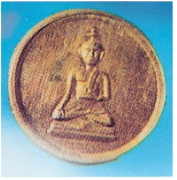
\includegraphics[scale=0.8]{images/art04-fn-20.jpg}} for Valluvar.

Missionaries in south used this Oriental research\index{Oriental research} on Linguistics to bring Race theory of Dravidian etc., and this still works in this part of India. As Thiruvalluvar has not used any names of Hindu gods, but only titles of attributes in first chapter "In praise of God" it became easy - but till date it survives and we need to verify this and explain why we say so.

\subsection*{Thirukkural as Jain Work – The False Claims}

Two major reasons put forth are

\begin{enumerate}[{\rm 1)}]
\itemsep=0pt
\item Thiruvalluvar \textbf{uses only titles of Based on attributes in his first Chapter “In praise of God"} and not names of deities. Now 10th century or later Tamil thesaurus (Nigandu\index{Nigandu}) mainly gives these attributes/ titles to Jain Thīrthankara.

 \item 
 Thiruvalluvar emphasis on Non-violence and not eating of meat is repeated emphasis on “Not killing"

 Main assumptions that help this thesis are the bogus commentaries of 20th century, most of which were written with the assumption of Aryan Invasion theories, which have been disproved.

 \item Valluvar is against Vedic rituals and against Varna system.

\end{enumerate}


\subsection*{Valluvar and Yajña}

Let us analyze this in the reverse two Kurals which are almost wrongly interpreted by most scholars

259. \textbf{Better than a thousand burnt Yajña offerings\supskpt{\endnote{259: \tamil{அவிசொரிந்து ஆயிரம் வேட்டலின் ஒன்றன் உயிர்செகுத்து உண்ணாமை நன்று.}}} Is one life un-killed, un-eaten.} (Abstinence from Flesh)

\textbf{Meaning} Not to kill and eat (the flesh of) an animal, is better than the pouring forth of ghee etc., doing a thousand YAGNAS.

Valluvar has given this Kural in abstinence from flesh- now what does he means here- You people do yajña-s to attain God - but if you eat flesh and you do not get any benefit once you eat flesh.

\textbf{The next Kural says} "All creatures will join their hands together, and worship him who has never taken away life, nor eaten flesh." - You yourself will be worshipped like God if you stop eating flesh.

\textbf{This Kural actually is in support of Yajña-s} and against flesh eating. All Valluvar says is that if one keeps on eating flesh there is no use in Yajña-s, which is the way to attain God. \textbf{Valluvar holds Yajña-s positively.}

Interestingly, Manu who promulgated animal sacrifice says in another place that one who abstains from meat obtains the same reward as one who does hundred years of horse-sacrifice (Manu Smŗti, V.53). This is similar to what Valluvar said.

So it is wrong to say that \textbf{Valluavar was against Vedic Yajña as it is opposite of what is said in Kural.}


\subsection*{False Claim - “Thiruvalluvar was agaist Brahmins by Birth”}

\endnote{30. \tamil{அந்தணர் என்போர் அறவோர்மற் றெவ்வுயிர்க்கும் செந்தண்மை பூண்டொழுக லான்.} Kural-30}\textbf{30 Ascetics} are called men of virtue for they assume The role of mercy to all that live. (30)

Meaning - The virtuous are truly called Anthanar\index{Anthanar} (Valluvar uses “Anthanar” here) because in their conduct towards all creatures they are clothed in kindness.

This chapter is "The Greatness of Ascetics" and here he refers Ascetics and nothing to do with Brahmins. Actually God, Sages are also called Anthanar in Sangam Literature and \textbf{hence here Valluvar talks about Sages and not Brahmins.}

 972. All human beings agree as regards their birth but differ as regards their characteristics, because of the different qualities of their actions.\endnote{\tamil{பிறப்பொக்கும் எல்லா உயிர்க்கும் சிறப்பொவ்வா செய்தொழில் வேற்றுமை யான்.}}

Now people are classified according to the nature of work they do- this indicates that Valluvar agrees with Varņāśrama\endnote{\tamil{வள்ளுவரும் சாதியும்- ஓர் உரையாடல்}

http://www.jeyamohan.in/20607\#.WakrOfMjHIU.}. But people stop with the first line alone while discussing this issue.


\subsection*{Valluvar clearly agrees – Varņa by birth}

134. Scriptures forgot can be recapitulated; Bad conduct debases a Brahmin and his birth.\endnote{\tamil{மறப்பினும் ஓத்துக் கொளல் ஆகும் பார்ப்பான் பிறப்பொழுக்கம் குன்றக் கெடும்}} - in chapter \tamil{ஒழுக்கமுடைமை.}- The Possession of Decorum

A Brahman though if he forgets the Veda-s may recover it; but, if he fails in propriety of conduct even his high birth will be destroyed.

120 As thriving trader is the trader known,\endnote{\tamil{வாணிகம் செய்வார்க்கு வாணிகம் பேணிப் பிறவும் தமபோல் செயின்} (\tamil{குறள்} – 120)}

\newpage

Who guards another's interests as his own. (\tamil{நடுவு நிலைமை.}- Impartiality)- \textbf{Here he refers to Vyśya-s as those who undertake trading.}

951.\endnote{95 - \tamil{இற்பிறந்தார் கண்அல்ல தில்லை இயல்பாகச் செப்பமும் நாணும் ஒருங்கு.} (951)} Consistency (of thought, word and deed) and fear (of sin) are conjointly natural only to the high-born. - \tamil{குடிமை} (nobility, civility citizenship)

952 \endnote{\tamil{ஒழுக்கமும் வாய்மையும் நாணும் இம் மூன்றும் இழுக்கார் குடிப்பிறந் தார்.} (952)}The high-born will never deviate from these three; good manners, truthfulness and modesty. 

\tamil{கயமை} (Inferiority, baseness, despicableness)

1075\endnote{1075 \tamil{அச்சமே கீழ்களது ஆசாரம் எச்சம் அவாவுண்டேல் உண்டாம் சிறிது}} (The principle of) behavior in the mean is chiefly fear; if not, hope of gain, to some extent. 

1078\endnote{\tamil{சொல்லப் பயன்படுவர் சான்றோர் கரும்புபோல் கொல்லப் பயன்படும் கீழ்} 1078} The great bestow (their alms) as soon as they are informed; (but) the mean, like the sugar-cane, only when they are tortured to death. 

1079\endnote{\tamil{உடுப்பதூஉம் உண்பதூஉம் காணின் பிறர்மேல் வடுக்காண வற்றாகும் கீழ்} 1079} The mean will bring an evil (accusation) against others, as soon as he sees them (enjoying) good food and clothing.


\subsection*{Basic Tenets of Jainism}

Life is spirit, not physical matter. Jainism is life-affirming, but world-denying. Jains reject a materialistic lifestyle.

Jainism is a religion which preaches Ascetics and all others to follow renunciation of Life, and important preachings of Jainism (Sannyāsi Dharma) compel seven rituals.

\begin{enumerate}[{\rm 1)}]
\itemsep=0pt
\item Kesa-lonch or Ulosam- While Taking Sanyāsam- need to pull all hairs individually and become bare-headed. Valluvar is against bare head and also too much growth. (Kural -280)
 
 \item Thihambaram (Digambara) - To Renounce clothing and Walking Nakedly. KURAL-1012 \& 788 tells us the importance of Dressing.
 
 \item 
 Asnana- (Not taking Bath)

 Valluvar even for Thurviyal says in Kural 298 the importance of bathing, and that Sanyāsin-s should take bath in Kural 278.

 \item 
 Bhūshayan - Sleep in Hard ground.

 Valluvar never says anything about sleeping on bare floor and at least he refers to soft bed in Kural 1191.

 \item 
 Adantdhavan – Not to wash teeth.

 In Kural 1121, when Valluvar refers clean Mouth- certainly he is for brushing teeth regularly.

 \item 
 Sthiti-bhojan (Eat while standing) –

 We do not find this in any of the Kurals at all.

 \item 
 Ekapuktham - Eating only once in a day.

 Valluvar has not said this anywhere, whereas he says that one must eat again after the earlier food has been digested i.e., within six hours.

 Valluvar’s way of Sanyāsa is not according to Jainism as he has not agreed with any of the above “Yati dharma”

\end{enumerate}


\subsection*{Valluvar and Ahimsā}

Two Chapters 25 "Abstainance of flesh" and 33 "Avoidance of killing " is under “Thuravaraviyal(Asceticism)”, but this is been excessively used to say that Valluvar’s main idea is this. Now on classification under Thuravaraviyal- as these researchers in their hypothesis say are not made by Valluvar but by later day copiers, but we can verify to whom Valluvar said this

258 \endnote{258: \tamil{செயிரின் தலைப்பிரிந்த காட்சியார் உண்ணார் உயிரின் தலைப்பிரிந்த ஊன்.}}\textbf{The wise, who have freed themselves from mental delusion}, will not eat the flesh which has been severed from an animal.

 325\endnote{325:\tamil{நிலைஅஞ்சி நீத்தாருள் எல்லாம் கொலைஅஞ்சிக் கொல்லாமை சூழ்வான் தலை.}} Of all those who, \textbf{fearing the permanence of earthly births, have abandoned desire}, he is the chief who, fearing (the guilt of) murder, considers how he may avoid the destruction of life.

328\endnote{328:. \tamil{நன்றாகும் ஆக்கம் பெரிதெனினும் சான்றோர்க்குக் கொன்றாகும் ஆக்கங் கடை.}} The advantage which might flow from destroying life in sacrifice, \textbf{is dishonourable to the wise (who renounced the world)}, even although it should be said to be productive of great good.

\textbf{These kurals clearly says that abstaining from flesh and killing are mainly advised for Ascetics.}

\textbf{Valluvar uses certain parables to illustrate his point.}

\textbf{Valluvar Refers Fishing and Cooking meat\index{meat} as Parables}

931: Don’t gamble even if you win for it draws you in \textbf{Like fishes drawn to shining baits.}

\textbf{Fish drawn in Bait- that is he refers to fishing for food for common man.}

1260. Is it possible for \textbf{those whose hearts melt like Mutton fat in the fire} to say they can feign a strong dislike and remain so?

Valluvar compares / explains the cooking of fat with the heart melting.


\subsection*{Agriculture \& Jainism}

Jainism is against agriculture as ploughing kills insects during agriculture\index{agriculture}, but Valluvar says that the farmer alone is the one really living independently and even ascetics depend on them.

1031\endnote{\tamil{சுழற்றும்ஏர்ப் பின்ன துலகம் அதனால் உழந்தும் உழவே தலை} (\tamil{குறள்} – 1031)} Agriculture, though laborious, is the most excellent (form of labour); for people, though they go about (in search of various employments), have at last to resort to the farmer.

1033\endnote{\tamil{உழுதுண்டு வாழ்வாரே வாழ்வார்மற் றெல்லாம் தொழுதுண்டு பின்செல் பவர்} (\tamil{குறள்} – 1033)} They alone live who live by agriculture; all others lead a cringing, dependent life.

1036 \endnote{1036: \tamil{உழவினார் கைம்மடங்கின் இல்லை விழைவதூஉம் விட்டேம்என் பார்க்கும் நிலை.}} If the farmer's hands are slackened, \textbf{even the ascetic state will fail.}


\subsection*{Thiruvalluvar and Family Life.}

In general, Jainism is a study in extremes: extreme atheism; extreme ahimsā; extreme asceticism

Jainism predominantly teaches to live as ascetics and renounce this life.

Women cannot achieve Mokṣa or liberation in this Life unless they do penance born again as male in Jainism. Valluvar\index{Valluvar} emphasis is on family life and says that family man is more important. 

Thiruvalluvar’s emphasis for Family life and Good Wife can be understood by separate chapters 5 \& 6.

6. The Good Wife’s Help

54. \endnote{\tamil{பெண்ணின் பெருந்தக்க யாவுள கற்பென்னும் திண்மைஉண் டாகப் பெறின்.}}What is more excellent than a wife, if she possess the stability of chastity?

Chapter 5. Family Life

46.\endnote{\tamil{அறத்தாற்றின் இல்வாழ்க்கை ஆற்றின் புறத்தாற்றில் போஒய்ப் பெறுவ தெவன்.}} What will he who lives virtuously in the domestic state gain by going into the other, (ascetic) state?

In Kural 50\endnote{\tamil{வையத்துள் வாழ்வாங்கு வாழ்பவன் வான்உறையும் தெய்வத்துள் வைக்கப் படும்.}}\textbf{He who on earth has lived in the conjugal state as he should live, will be placed among the Gods who dwell in heaven.}

Chapter - \textbf{Wealth That Benefits None}

1007\endnote{1007 \tamil{அற்றார்க்கொன்று ஆற்றாதான் செல்வம் மிகநலம் பெற்றாள் தமியள்மூத் தற்று}} The wealth of him who never bestows anything on the destitute is like a woman of beauty growing old without a husband.

Life of ascetism is even criticised as a beautiful women wasting life without marrying and no family life. Jainism predominantly teaches detachment and abstinence from this worldly pleasures and Valluvar writes for earthly life with good virtues. Jains reject materialistic lifestyle.


\section*{5 Names of God in First Chapter}

Thirukkural belongs to the period of late 3rd Century or early 4th and we see the nature of literature composed was more didactic compared to that of Sangam\index{Sangam} period, which was more lively; the land was ruled by Kalappirar \textbf{who were mostly} Jains and perhaps Valluvar had to adapt his style due to this reason.

Now of all the titles used

\tamil{ஆதி பகவன்} (First Creator god)

Saiva Saint Thirugnana \textit{Sambandhar}\index{Sambandhar@\textit{Sambandhar}} uses similar term in Devaram 1:88:5

\tamil{வாலறிவன்} (Pure intelligence)

Saiva Saint Thirugnana Sambandar uses similar meant title in Devaram\index{Tevaram} 1:69:3

\tamil{மலர்மிசை ஏகினான்} (One who walked on flowers)

Saiva Saint Thirugnana Sambandar uses similar meant title in \textit{Devaram}\index{Tevaram} 1:21:5

\tamil{வேண்டுதல் வேண்டாமைஇலான்} (One who is beyond likes and dislikes)

\tamil{இறைவன்} (God)

\tamil{ஐந்தவித்தான்} (One who controlled five senses) 3:319:7

\tamil{தனக்குவமை இல்லாதான்} (One beyond compare) 2:198:3

\tamil{அறவாழி அந்தனன்} (One with sea or wheel of virtue) 1:9:2, 2:199:11

\tamil{எண் குணத்தான்} (One with 8 attributes)

\tamil{இறைவன்} (God)

Thiruvalluvar refers to Lord Almighty Creator of Universe - and not a Saintly man when he says - One beyond compare, One who is beyond likes and dislikes, Lord \& First Creator god. Few of the other titles could appear as it refers to a ascetic - but one can be certain Valluvar was talking about Creator God and not any Human Ascetic as it appears. Most of this has been used by Devarams of 7th century for Śiva- which was much earlier to Tamil Nigandus mostly written by Jains.

Calling God as Vedic is never in practice in Jainism in First Millennium, whereas it can be seen in Paripāḍal for Lord Brahma and\endnote{\tamil{ஆதி அந்தணன் அறிந்து பரி கொளுவ - பரி} 5/22\\\tamil{இமைய வில் வாங்கிய ஈர்ம் சடை அந்தணன்/உமை அமர்ந்து உயர் மலை இருந்தனன் ஆக - கலி} 38/1,2\\\tamil{மலர்மிசை முதல்வனும், மற்று அவனிடைத் தோன்றி பரி} 8:3} Lord Shiva in Kalithogai.

Valluvar has given more importance to Family life- he allocated 22 Chapters over Asceticism for which he allocates 15 Chapters. The Virtues for Asceticism for Jain monks have all been negated by Valluvar as can be seen above.

We began this elaborate exercise to find answers to the following questions:

\begin{itemize}
\item If the morals taught by Valluvar in Kuŗal are based on Sanātana Dharma\index{Sanatana Dharma@Sanātana Dharma}, most of which could be common with other religions but Valluvar goes against Jainism clearly

 \item If the Deity praised by Valluvar in his first chapter is the Creator God then it is not acceptable to Jainism.

\end{itemize}

We compared the principal teachings of Valluvar to the then philosophical traditions that prevailed during the times of Valluvar. Then we compared the contents of the Kuŗal with some ethical treatises in Brahminic Hinduism, Buddhism and Jainism. We also looked at Valluvar's references to "God and gods" in light of the concept of god in Jainism. And finally, we made a detailed investigation of every couplet of the first chapter and tried to relate the names and attributes employed by Valluvar\index{Valluvar} to deities in Buddhism, Christianity, Jainism, Vaishnavism and Saivism.

One cannot reject or accept the claims of religious affiliation of a book based on the mere presence of one or two verses in support or against a particular faith. Evidences have to be rather consistent and distributed throughout the work. No doubt the Kuŗal\index{Kuŗal@Kuŗal} has many references to Hinduism, Jaina, and Buddhist beliefs. However, such passing references cannot be taken as indication of the author's affiliation or inclination to any particular faith because such references have been found across literary works of known affiliation to all the three religious systems of Jainism, Buddhism and Hinduism.

However Valluvar’s idea of Creator God and positive (materialistic) life on Earth are totally against Jainism.

\subsection*{Valluvar and Vedic Dharma Śāstra-s}

Valluvar teaches in his section on Politics as to how a King must rule a land

543.\endnote{543:.\tamil{அந்தணர் நூற்கும் அறத்திற்கும் ஆதியாய் நின்றது மன்னவன் கோல்.}} The \textbf{sceptre of the king is the firm support of the Vedas of the Brahmin}, and of all virtues therein described. \textbf{(Just Reign)}

Now this can be clearly understood when you compare with Silapathikaram\endnote{\tamil{சிலப்பதிகாரம் அடைக்கலக் காதை}\\\tamil{“கடவது அன்றுநின் கைத் தூஉண் வாழ்க்கை;}\\\tamil{வடமொழி வாசகம் செய்த நல்லேடு}\\\tamil{கடனறி மாந்தர் கைந்நீ கொடுக்க” என.....” (அடைக்கலக் காதை)}} in which a Brahim wife who killed mongoose and on her plea her husband wrote the penance methods and gifts to be given, on a sheet; \textbf{Kovalan\index{Kovalan} the Vyśya read that Sanskrit sūtra-s} and helped the Brahmin woman to achieve the penance.

\textbf{Unjust Reign}

560 \endnote{560:.\tamil{ஆபயன் குன்றும் அறுதொழிலோர் நூல்மறப்பர் காவலன் காவான் எனின்.}} If the guardian (of the country) neglects to guard it, the produce of the cows will fail, and the men of six duties viz., the Brahmins will forget the Veda-s.

In the Chapter 2- \textbf{Importance of Rain}, Valluvar says

\textbf{18. If the heaven dry up, neither yearly festivals, nor daily worship will be offered in this world, to the celestials.}

\textbf{Now, what if a King is bad:-}

\textbf{559.\supskpt{\endnote{\tamil{முறைகோடி மன்னவன் செய்யின் உறைகோடி ஒல்லாது வானம் பெயல்.}}} If the king acts contrary to justice, rain will become unseasonal, and the heavens will withhold their showers.}

\textbf{In the previous verses Valluvar says that if the king acts contrary to justice, rain will become unseasonal, and the heavens will withhold their showers. This indicates that for Valluvar, Brahmins forgetting Veda-s is much worse than the rains being withheld by the heavens.}

\endnote{28.\tamil{நிறைமொழி மாந்தர் பெருமை நிலத்து மறைமொழி காட்டி விடும்.}} 28. The hidden words of the men whose words are full of effect (Vedas), will show their greatness to the world.

\textbf{The Veda-s are called Śruti meant heard and not to be written, and in Tamil it is so called “MARAI" means hidden or un-written.}

\textbf{Valluvar calls Veda-s by Another name \tamil{“ஓத்து"} this word is very special Veda-s are always passed on by Guru Paramparā and said jointly - in \textit{Tamil}\index{Tamil} \tamil{“ஓது"} means read but as Veda-s are recited verbally only; mostly simultaneously recited (\tamil{ஒத்து}) in a meter}

\textbf{(Chandas) so it is \tamil{“ஓத்து"}}

\textbf{Valluvar has used many Sanskrit verses From \textit{Manusmŗti}\index{Manusmrti@\textit{Manusmŗti}}, \textit{Dharma Śāstra}-s\index{Dharma Sastra@\textit{Dharma Śāstra}} \textit{Mahābhārata}\index{Mahabharata@\textit{Mahābhārata}} etc., and also from Buddhistic and Jain Sāstra-s.}

\textbf{Valluvar in his chapter 4 on Domestic Life}

\textbf{43. \supskpt{\endnote{\tamil{தென்புலத்தார் தெய்வம் விருந்தொக்கல் தானென்றாங்கு ஐம்புலத்தாறு ஓம்பல் தலை.} (43)}}A householder's main duty is to serve these five: Ancestors, God, guests, kindred, and himself.}

This is also said in Mahābhārata and Śatapatha Brāhmaņa.

There are five great sacrifices, namely, the great ritual sacrifices: The sacrifice to all beings, sacrifice to me, sacrifice to the ancestors, Sacrifice to the gods, sacrifice to Brahman. \textbf{(Śatapatha Brāhmaņa 11.5.6.1)}

\textbf{This order is very important.}

Ancestors first, next God, the worship of Pitŗ-s or ancestors takes importance over God, during every New Moon day People do Tarpaņa and annual Śrāddha and Mahālaya Amāvāsya etc. During these days the couple performing ceremony to ancestors should not visit temple or undertake pūja-s also. For one year from the death of close ancestor the orthodox do not visit temple or celebrate any festivals. Pitŗ Yajña is most important over even God.


\subsection*{Valluvar and Family Man}

41.\endnote{\tamil{இல்வாழ்வான் என்பான் இயல்புடைய மூவர்க்கும் நல்லாற்றின் நின்ற துணை.} (41)} A householder is a steadfast friend to the other three orders in their virtuous paths.

Here Valluvar says the Family Man (Gŗhastha) should take care of other three- Brahmacārin-s, Vanaprastha-s and Sanyāsin-s.

\textbf{Valluvar\index{Valluvar} uses names of Gods in many Kurals and few are as below.}

Lord Vishnu and Lakshmi in - 84, 167, 179, 519, 617, 920, 1103\\ Bhoomidevi-1040\\ Srashta Devi or Elder of Laksmi- 167, 617, 936\\ Indra -25,899\\ Lord Brahma – 1062\\ Manmatha -1197\\ Yama: 269, 326, 765, 894, 1050, 1083, 1085

Like Lajja in \tamil{நாணெணும் நல்லாள்} (924) and Thara \tamil{நிலமெனும் நல்லாள்} (1040)

And many “See Lord Shiva Drinking Poison” is referred in Kural 355

When the Indian Government wanted to release commemorative Stamp and Coin in Honour of Thiruvalluvar and asked to give image of Valluvar, as per the Speech on 2011 for Thiruvalluvar day awards on 16th January by the then Chief Minister M. Karunanidhi\endnote{50 \url{ http://www.dinamalar.com/news_detail.asp?Id=167478&Print=1} - \tamil{சிலருக்கு குறை இருந்தது.வள்ளுவர் பிராமணராக இருந்ததால் தான் அவரால் இத்தகைய திருக்குறளை இயற்ற முடிந்தது. அவர் சாதாரணமாக இருந்திருக்க முடியாது என, சிலர் பேசிக் கொண்டனர். திருவள்ளுவர் உடலில் பூணூல் இருக்க வேண்டுமென அவர்கள் கேட்டுக் கொண்டனர். இதனால், பிரச்னை ஏற்படாமல் இருக்க, ஓவியர் வேணுகோபால் சர்மா, திருவள்ளுவர் சால்வையை போர்த்தியிருப்பது போல, வள்ளுவர் படத்தை வரைந்து கொடுத்தார்.}}\index{Karunanidhi, M.} many Scholars felt that Thiruvalluvar was a Brahmin as he has adopted many Sanskrit verses and translated them in Tamil and hence the picture of Valluvar must have Sacred Pūņal (sacred thread\index{sacred thread}). Then came the idea of a shawl covering the body.

Valluvar has extensively used Sanskrit verses from Manusmŗti\index{Manusmrti@Manusmŗti}, Mahābhāratha\index{Mahabharatha@Mahābhāratha}, Bhagavad Gītā\index{Bhagavad Gita@Bhagavad Gītā} and also from Jain \textit{Suktham} and \textit{Dhamma padam} of Buddhists.

Valluvar’s Thirukkural is not a religious work – but is meant to teach virtues. His ideas on ascetism are against those of Jainism; Valluvar asks us to follow Creator God and pursue positive earthly life -- all this are the tenets of Sanātana Dharma\index{Sanatana Dharma@Sanātana Dharma}.

\newpage

\theendnotes

